\documentclass[tikz,border=2pt]{standalone}
% shared tikz preamble for generating svg figures
% keep this file minimal; figure-specific styles can live in the figure .tex if needed
\usepackage{tikz}
\usetikzlibrary{positioning}
\usetikzlibrary{shapes.geometric}
\usetikzlibrary{arrows}
\usetikzlibrary{decorations}
\usetikzlibrary{decorations.markings}

\tikzset{>=latex}
\tikzstyle{Arrow} = [->, thin, preaction = {decorate}]
\tikzstyle{cor} = [-, dotted, preaction = {decorate}]

\begin{document}
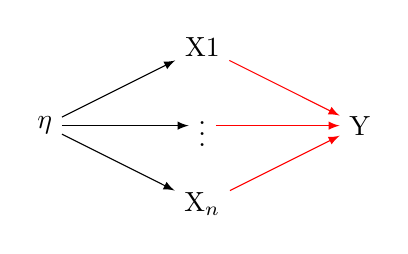
\begin{tikzpicture}[{every node/.append style}=draw]
\node [rectangle, draw=white] (eta) at (2, 0) {$\eta$};
\node [rectangle, draw=white] (X1) at (4, 1) {X1};
\node [rectangle, draw=white] (X2) at (4, 0) {$\vdots$};
\node [rectangle, draw=white] (Xn) at (4, -1) {X$_n$};
\node [rectangle, draw=white] (Y) at (6, 0) {Y};

\draw [-latex, draw=black] (eta) to (X1);
\draw [-latex, draw=black] (eta) to (X2);
\draw [-latex, draw=black] (eta) to (Xn);

\draw [-latex, draw=red] (X1) to (Y);
\draw [-latex, draw=red] (X2) to (Y);
\draw [-latex, draw=red] (Xn) to (Y);
\end{tikzpicture}
\end{document}
